\documentclass[11pt, a4paper]{article}

% ── Packages
\usepackage[margin=1in]{geometry}
\usepackage{amsmath, amssymb}
\usepackage{listings}
\usepackage{xcolor}
\usepackage{enumitem}
\usepackage{tikz}
\usetikzlibrary{calc, positioning}
\usepackage{fancyhdr}
\usepackage{titlesec}
\usepackage{hyperref}

% ── Colors
\definecolor{uwmuted}{HTML}{6B7280}
\definecolor{codebg}{HTML}{1E1E1E}
\definecolor{codecomment}{HTML}{6A9955}
\definecolor{codekeyword}{HTML}{569CD6}
\definecolor{codetype}{HTML}{4EC9B0}
\definecolor{codetext}{HTML}{D4D4D4}
\definecolor{stencilblue}{HTML}{3B8BD4}
\definecolor{stencilcoral}{HTML}{D85A30}

% ── Code listing style
\definecolor{linenogray}{HTML}{555555}

\lstdefinestyle{cppstyle}{
    language=C++,
    basicstyle=\ttfamily\footnotesize\color{codetext}\linespread{1.15}\selectfont,
    backgroundcolor=\color{codebg},
    keywordstyle=\color{codekeyword},
    commentstyle=\itshape\color{codecomment},
    morekeywords={size_t, constexpr, nullptr, auto},
    emphstyle=\color{codetype},
    emph={Grid},
    breaklines=true,
    showstringspaces=false,
    tabsize=4,
    frame=single,
    rulecolor=\color{codebg},
    xleftmargin=2em,
    xrightmargin=1em,
    aboveskip=1em,
    belowskip=0.8em,
    framesep=0.8em,
    framexleftmargin=1.5em,
    numbers=left,
    numberstyle=\tiny\ttfamily\color{linenogray},
    numbersep=10pt,
}

\lstdefinestyle{cppinterface}{
    style=cppstyle,
    numbers=none,
    xleftmargin=1em,
    framexleftmargin=0.5em,
}
\lstset{style=cppstyle}

% ── Inline code
\newcommand{\code}[1]{\texttt{#1}}

% ── Section formatting 
\titleformat{\section}{\large\bfseries}{}{0em}{}[\vspace{-0.3em}\rule{\textwidth}{0.4pt}]
\titleformat{\subsection}{\normalsize\bfseries}{}{0em}{}

% ── Header/Footer
\pagestyle{fancy}
\fancyhf{}
\fancyhead[L]{\small\textbf{UWHPC}}
\fancyhead[R]{\small\textcolor{uwmuted}{2D Heat Diffusion}}
\fancyfoot[C]{\small\thepage}
\renewcommand{\headrulewidth}{0.4pt}

% ── Document
\begin{document}

\begin{center}
    {\LARGE\bfseries Onboarding Problem}\\[0.4em]
    {\large 2D Heat Diffusion on a Uniform Grid}\\[0.8em]
    {\small\textcolor{uwmuted}{University of Waterloo High-Performance Computing Team}}\\[0.3em]
\end{center}

\vspace{1.5em}

\section{Overview}

You will implement two components of a 2D heat diffusion solver:
\begin{enumerate}[leftmargin=1.5em, itemsep=0.3em]
    \item A \textbf{grid class} that stores the 2D temperature field in memory.
    \item The \textbf{stencil kernel} that advances the simulation by one time step.
\end{enumerate}
Everything else, i.e., the time integrator, boundary conditions, initial conditions, and I/O, is provided. You DO NOT need to know any thermal physics or theory.

\section{The Math}

\subsection{The Governing Heat Equation}

Heat spreads across a 2D surface according to the following Partial Differential Equation:
\begin{equation}
    \frac{\partial T}{\partial t} \;=\; \alpha \left( \frac{\partial^2 T}{\partial x^2} + \frac{\partial^2 T}{\partial y^2} \right)
\end{equation}
where $T(x,y,t)$ is the temperature and $\alpha$ is a constant. Again, you do not need to understand the physics, math, theory, or origin of the equation; this is merely for context.

\subsection{Discretization onto a Grid}

Replace the continuous derivatives with finite differences:
{\small
\begin{equation}
    T_{t+1}(i,j) = T_t(i,j) + \Delta t \cdot \alpha \!\left( \frac{T_t(i{+}1,j) - 2T_t(i,j) + T_t(i{-}1,j)}{\Delta x^2} + \frac{T_t(i,j{+}1) - 2T_t(i,j) + T_t(i,j{-}1)}{\Delta y^2} \right)
\end{equation}
}

\subsection{Given Constants}

With constants $\alpha$, $\Delta x$, $\Delta y$, and $\Delta t$ chosen for stability, the equation simplifies to the following:
\begin{equation}
\boxed{\;T_{t+1}(i,j) \;=\; 0.5 \cdot T_t(i,j) \;+\; 0.125 \cdot \bigl( T_t(i{-}1,j) + T_t(i{+}1,j) + T_t(i,j{-}1) + T_t(i,j{+}1) \bigr)\;}
\end{equation}

\subsection{Converting Equations to Code}

Notice how this is just a weighted average. In code, the above could look something like this:
\begin{lstlisting}
new_arr[i][j] = 0.5   *  old_arr[i][j] +
                0.125 * (old_arr[i-1][j] + 
                         old_arr[i+1][j] + 
                         old_arr[i][j-1] + 
                         old_arr[i][j+1]
                        );
\end{lstlisting}

\subsection{The Five-Point Stencil}

To provide a more visual understanding and intuition of what is happening, consider the diagram below. You can picture the heat from each "bubble" (grid cell) leaking into its neighbors.
\begin{center}
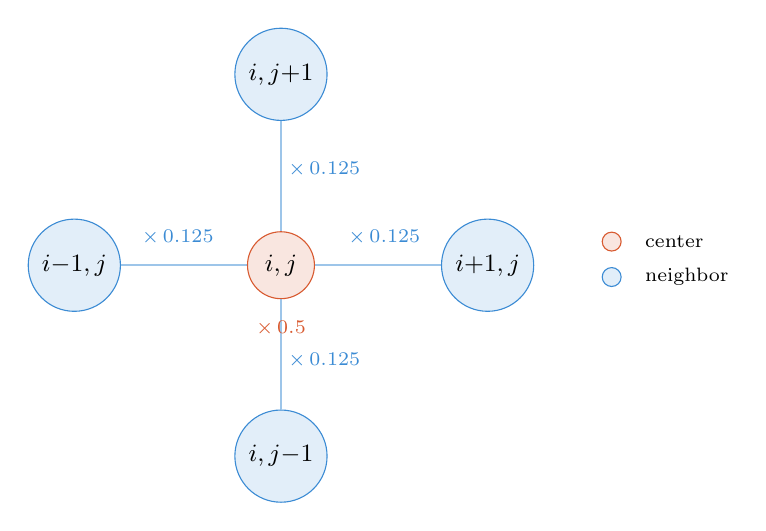
\begin{tikzpicture}[
    neighbor/.style={circle, draw=stencilblue, fill=stencilblue!15,
                     minimum size=0.7cm, font=\small},
    center/.style={circle, draw=stencilcoral, fill=stencilcoral!15,
                   minimum size=0.85cm, font=\small\bfseries},
]
    % Nodes
    \node[center]   (c) {$i,j$};
    \node[neighbor] (n) [above=1.4cm of c] {$i,j{+}1$};
    \node[neighbor] (s) [below=1.4cm of c] {$i,j{-}1$};
    \node[neighbor] (w) [left=1.6cm of c]  {$i{-}1,j$};
    \node[neighbor] (e) [right=1.6cm of c] {$i{+}1,j$};

    % Edges
    \draw[stencilblue, thick, opacity=0.5] (n) -- (c);
    \draw[stencilblue, thick, opacity=0.5] (s) -- (c);
    \draw[stencilblue, thick, opacity=0.5] (w) -- (c);
    \draw[stencilblue, thick, opacity=0.5] (e) -- (c);

    % Weight labels
    \node[font=\scriptsize, stencilblue]
        at ($(c)!0.5!(n) + (0.55, 0)$) {$\times\, 0.125$};
    \node[font=\scriptsize, stencilblue]
        at ($(c)!0.5!(s) + (0.55, 0)$) {$\times\, 0.125$};
    \node[font=\scriptsize, stencilblue]
        at ($(c)!0.5!(w) + (0, 0.35)$) {$\times\, 0.125$};
    \node[font=\scriptsize, stencilblue]
        at ($(c)!0.5!(e) + (0, 0.35)$) {$\times\, 0.125$};
    \node[font=\scriptsize, stencilcoral, below=0.15cm of c]
        {$\times\, 0.5$};

    % Legend
    \draw[fill=stencilcoral!15, draw=stencilcoral]
        (4.2, 0.3) circle (0.12cm);
    \node[anchor=west, font=\scriptsize] at (4.5, 0.3) {center};
    \draw[fill=stencilblue!15, draw=stencilblue]
        (4.2, -0.15) circle (0.12cm);
    \node[anchor=west, font=\scriptsize] at (4.5, -0.15) {neighbor};
\end{tikzpicture}
\end{center}

\section{Task 1: The Grid Class}

Design and implement a \code{Grid} class that stores a 2D field of \code{double} values of size $N_x \times N_y$. While you may expand as much as you wish, your class must satisfy the following interface:

\begin{lstlisting}[style=cppinterface]
#include <cstddef>

class Grid {
private:
    std::size_t Nx_;
    std::size_t Ny_;

public:
    Grid(std::size_t nx, std::size_t ny);

    std::size_t Nx() const;
    std::size_t Ny() const;

    // Element access -- you must implement both overloads.
    double& operator()(std::size_t i, std::size_t j);       // read/write
    double  operator()(std::size_t i, std::size_t j) const; // read
};
\end{lstlisting}

The two \code{operator()} overloads give read/write and read-only access to the cell at row \code{i}, column \code{j}. The evaluation harness uses them---and only them---to set initial conditions and read back your results, so they must work no matter how you store the field internally. Everything behind this interface is up to you. We want to see how you think and how you approach such problems.

\vspace{6pt}

\noindent \textbf{Requirements}:
\begin{enumerate}[leftmargin=1.5em, itemsep=0.2em]
    \item Default-initialized to zero.
    \item Implement both \code{operator()} overloads; the evaluation harness relies on them.
    \item You choose the memory layout behind that interface. You will be asked to justify your choice.
\end{enumerate}

\section{Task 2: The Stencil Kernel}

Implement the function that applies the five-point stencil over all interior grid points ($1 \leq i < N_x - 1$, $\; 1 \leq j < N_y - 1$).

Boundary values must remain unchanged. You are not required to implement any boundary conditions; simply copy the boundary values from the old grid to the new grid.

\noindent The boundary copy below is illustrative; the interior update is yours to write.

\begin{lstlisting}[style=cppinterface]
void apply_stencil(const Grid& old_grid, Grid& new_grid) {
    // Copy boundaries
    for (std::size_t i{}; i < old_grid.Nx(); ++i) {
        new_grid(i, 0) = old_grid(i, 0);
        new_grid(i, old_grid.Ny() - 1) = old_grid(i, old_grid.Ny() - 1);
    }

    for (std::size_t j{}; j < old_grid.Ny(); ++j) {
        new_grid(0, j) = old_grid(0, j);
        new_grid(old_grid.Nx() - 1, j) = old_grid(old_grid.Nx() - 1, j);
    }

    // Your implementation...
}
\end{lstlisting}

\section{Deliverables}
 
\begin{enumerate}[leftmargin=1.5em, itemsep=0.2em]
    \item \code{grid.hpp} --- the \code{Grid} class.
    \item \code{stencil.cpp} --- the \code{apply\_stencil} function.
\end{enumerate}
 
\section{Evaluation}
 
\begin{center}
\renewcommand{\arraystretch}{1.3}
\begin{tabular}{l l}
    \textbf{Correctness} & Output matches reference within $10^{-10}$ per grid point. \\
    \textbf{Performance} & Wall-clock time on the team benchmark machine. \\
    \textbf{Code quality} & Clean C++17. \\
\end{tabular}
\end{center}

We will be selective in evaluating implementations. Note that correctness alone is not sufficient; we expect thoughtful consideration of performance, memory layout, and overall design.

\section{Submission}

Submit your \code{grid.hpp} and \code{stencil.cpp}. After your submission, we will invite you to a short virtual chat to discuss your design and the choices you made.

\section{On Artificial Intelligence}

We encourage using AI to learn and explore ideas. That said, your submission should be your own work; copy-pasting from AI will be obvious, especially during the chat.
 
\vspace{1.5em}
 
\begin{center}
    \textcolor{uwmuted}{\small Good luck.}
\end{center}
 
\end{document}